% Exact hook-walk probabilities for shape (3,1).
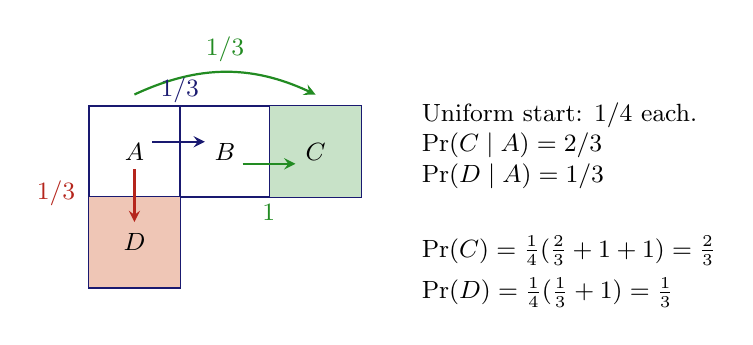
\begin{tikzpicture}[font=\small,>=stealth]
\foreach \j in {0,1,2}{\draw[MidnightBlue,thick] (1.15*\j,0) rectangle (1.15*\j+1.15,-1.15);}
\draw[MidnightBlue,thick] (0,-1.15) rectangle (1.15,-2.3);
\fill[ForestGreen!25] (2.3,0) rectangle (3.45,-1.15);
\fill[BrickRed!20] (0,-1.15) rectangle (1.15,-2.3);
\node at (0.575,-0.575) {$A$};
\node at (1.725,-0.575) {$B$};
\node at (2.875,-0.575) {$C$};
\node at (0.575,-1.725) {$D$};
\draw[->,thick,BrickRed] (0.575,-0.8) -- (0.575,-1.47);
\draw[->,thick,MidnightBlue] (0.8,-0.45) -- (1.47,-0.45);
\draw[->,thick,ForestGreen] (0.575,0.15) to[bend left=25] node[above] {$1/3$} (2.875,0.15);
\draw[->,thick,ForestGreen] (1.95,-0.73) -- (2.62,-0.73);
\node[BrickRed] at (-0.42,-1.1) {$1/3$};
\node[MidnightBlue] at (1.15,0.2) {$1/3$};
\node[ForestGreen] at (2.28,-1.35) {$1$};
\node[anchor=west,align=left] at (4.1,-0.5) {Uniform start: $1/4$ each.\\$\Pr(C\mid A)=2/3$\\$\Pr(D\mid A)=1/3$};
\node[anchor=west,align=left] at (4.1,-2.1) {$\Pr(C)=\frac14(\frac23+1+1)=\frac23$\\[4pt]$\Pr(D)=\frac14(\frac13+1)=\frac13$};
\end{tikzpicture}
